\subsection*{Übertragungsmedien}

\begin{example2}{Berechnung Signaldämpfung}\\
    \includegraphics[width=0.75\linewidth]{images/example_signaldämpfung.png}
    $$U1/U2 = 1/0.5 = 2, Signaldämpfung = 20 \cdot log(2) = 6dB$$
\end{example2}

\subsubsection{Strukturierte Gebäudeverkabelung nach ISO/IEC 11801}
        \centering
        \includegraphics[width=1\linewidth]{images/Gebäudeverkabelung.png}

\subsection*{Physical Layer}

\begin{example}
    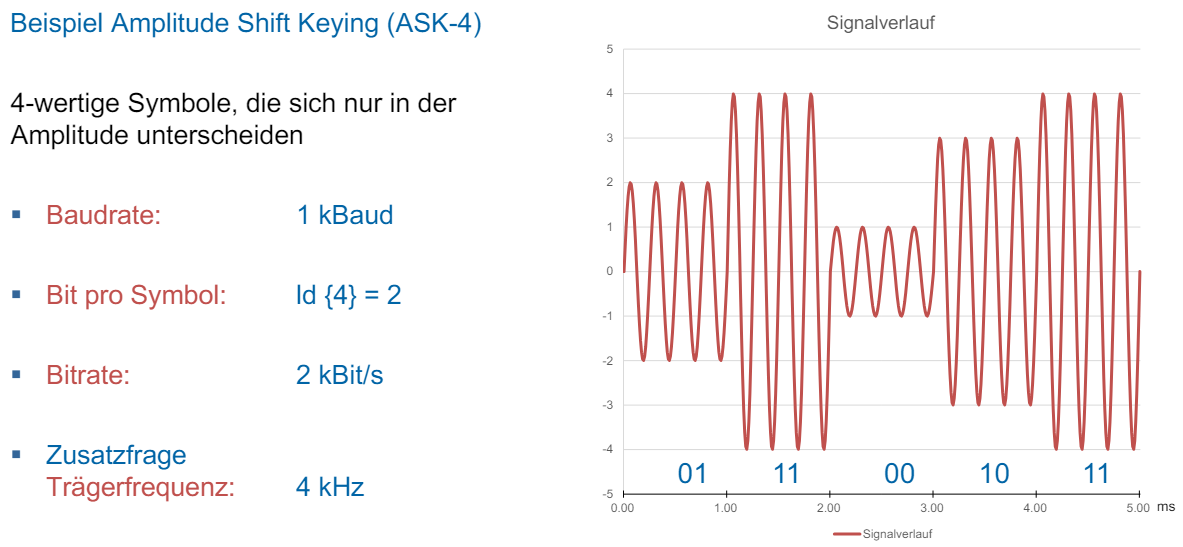
\includegraphics[width=1\linewidth]{images/amplitude_shift_keying.png}
\end{example}

\begin{concept}{AMI Leitungscode}\\
    3-wertiger AMI-Code (Alternate Mark Inversion)\\
    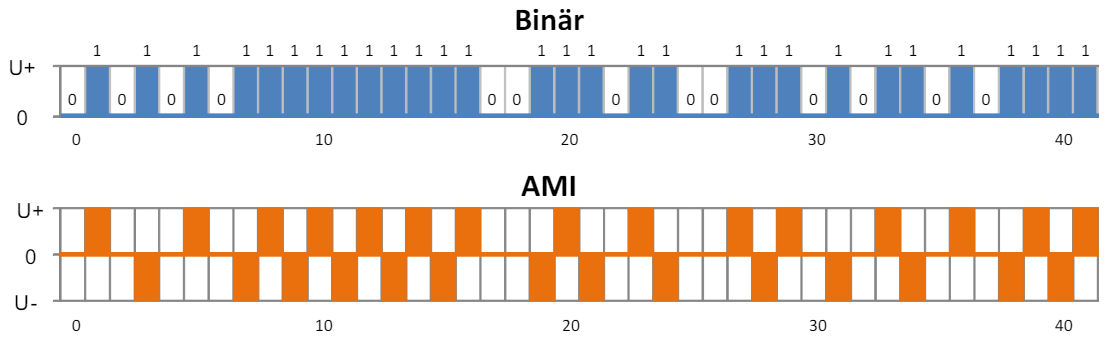
\includegraphics[width=0.8\linewidth]{images/gleichspannungsfreiheit.png}\\
    Nachteile dieses Leitungscodes:
    \begin{itemize}
        \item Auf der Übertragungsstrecke drei Zustände benötigt $\rightarrow$ rein binäre Medien genügen nicht
        \item Bei einer längeren Folge von 0 in den Daten ist keine Taktrückgewinnung mehr möglich
    \end{itemize}
\end{concept}

\begin{concept}{Manchester Leitungscode}\\
    wird z.B. bei 10BASE-T Ethernet verwendet, erlaubt einfache Taktrückgewinnung
    \begin{itemize}
        \item 1 positive Flanke, 0 negative Flanke
        \item Bei jedem Bit gibt es einen Signalwechsel
        \item Bandbreite von 10 MHz benötigt (2 $\times$ theoretisches Minimum)
    \end{itemize}
    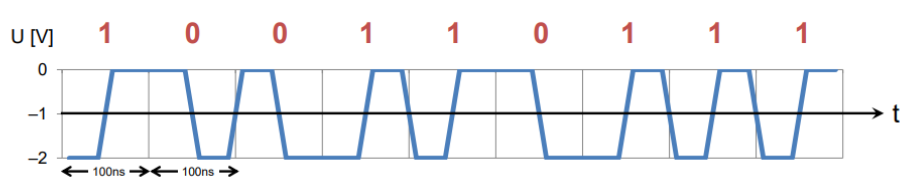
\includegraphics[width=0.6\linewidth]{images/leitungscode.png}
\end{concept}

\begin{concept}{NRZI MLT-3 Leitungscodierung}\\
    NRZI-Codierung (Non Return to Zero Inverted), kombiniert mit MLT-3\\
        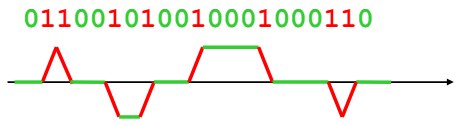
\includegraphics[width=0.5\linewidth]{images/leitungscodierung.png}\\
    MLT-3 = Multi-Level Transmit - Ternary
\end{concept}

\subsection*{Data Link Layer}

\begin{example}
    Gegeben: Bitrate 100 Mbit/s, Frame-Länge 1000 Byte, IFG 96 Bit, Payload 800 Byte. Berechnen Sie die Nutzdatenrate.\\
    \textbf{Lösung:}\\
    $$F_R = \frac{100 \cdot 10^6}{8 \cdot (1000 + 96)} = 1.19 \cdot 10^6 \text{ Frames/s}$$
    $$N = 1.19 \cdot 10^6 \cdot 800 \cdot 8 = 7.6 \cdot 10^9 \text{ Bit/s} = 7.6 \text{ Gbit/s}$$
\end{example}

\subsubsection*{LAN und Ethernet}

\begin{formula}{GBASE-T}\\
    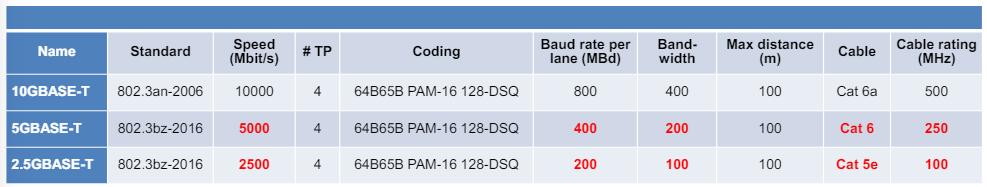
\includegraphics[width=1\linewidth]{images/GBASE-T.png}
\end{formula}